\chapter{Signalverarbeitung bei ballistokardiographischen Signalen}

\section{Grundsätzliches}

\begin{itemize}
	\item Signale sind durch quasiperiodische Natur des Herzens selbst quasiperiodisch
	\item gleichzeitige Messung von zwei verschiedenen Vorgängen gleichzeitig
	\item Morphologie variiert im Verlauf eines Atemzyklus
	\item Filterung nach Frequenzen durch Bandpass-Filterung möglich
	\item Normbereich Atemfrequenz: 12 bis 25 Atemzüge pro Minute, ober- und unterhalb abnormal
	\item Herzfrequenz: 30 bis 210 Schläge pro Minute, dabei 30 Schläge pro Minute Pulsabsenkung nachts, Ruhepuls ist höher
	\item durch Eigenschaften von \ac{BKG}-Signalen schwieriger in Signalverarbeitung als andere kardiorespiratorische Signale
	\item \citeauthor{Paalasmaa2015} Zitat:
\end{itemize}

\begin{quote}\textit{The properties of the BCG signal vary so much in practice that no simple filtering rule can be devised for an accurate and reliable beat-to-beat interval detection}\footcite{Paalasmaa2015}\end{quote}

\begin{itemize}
	\item verschiedene Arten Signalverarbeitung: Arbeit im Zeitbereich, Arbeit im Frequenzbereich
	\item Zeitbereich: oft basierend auf existierendem Wissen über Morphologie des physiologischen Signals -> bei \ac{BKG} schwierig, da Morphologie sehr variabel
	\item frequenzbasiert: Analyse von spektralen Eigenschaften
	\item Analysen im Frequenzbereich erstmal nur durchschnittliche Frequenzen
	\item für einige medizinsche Anwendungen ausreichend, für andere, zB \ac{HRV} nicht
\end{itemize}

\section{Detektion von Herzschlägen}\label{CLIE}

	\begin{itemize}
		\item in dieser Arbeit Fokus auf von Brüser entwickelter Algoritmus, dem \textit{Continuous Local Interval Estimator}, kurz \textit{CLIE}
		\item in \ref{ballistokardiographie} erwähnte Annahme: aufeinander folgende Herzschläge ähneln sich
		\item Vorverarbeitung: Bandpass-Filter 0.5 und 20 Hz
		\item erste Ableitung des mit Savitzky-Golay gefilterten Signals für Analyse genutzte
		\item Algorithmus iteriert mit \textit{Moving Window} über das Signal
		\item 2 Schwellwerte genutzt, $T_min$ und $T_max$, basierend auf bekanntem Bereich der Herzrate
		\item Fensterlänge 2 mal maximale Intervalllänge \[w_i[v] = x[n_i + v], v \in \{ -T_{max} * f_s, ..., T_{max} * f_s\} \]
		\item adaptives Fenster schätzt nur Intervalllänge an Mittelpunkt des Fensters
		\item lokale Intervalllänge $T_i$ schätzen
		\item Zentrum des Analysefensters weiter bewegen $n_{i+1} = n_i + \Delta t * f_s$
		\item Schätzung der Intervalllänge durch drei Schätzer
	\end{itemize}
	
	\begin{align*}
		E\textsubscript{Corr}[n] &= \frac{1}{n} \sum_{v=0}^{n} w[v]w[v-n],\\
		E\textsubscript{AMDF}[n] &= (\frac{1}{n} \sum_{v=0}^{n} |w[v]-w[v-n]|)^{-1},\\
		E\textsubscript{MAP}[n] &= \max_{v \in \{0,...,n\}}(w[v]+w[v-n]).
	\end{align*}
	
	\begin{itemize}
		\item $E_{corr}$ berechnet eine modifizierte Autokorrelationsfunktion, mit $E_{AMDF}$ wird die Differenz des Signals zueinander miteinbezogen, AMDF steht für Modified average magnitude difference function
		\item mit $E_{MAP}$ werden die maximale Amplituden von beliebigen 2 Samples über das ganze Fenster berechnet, MAP steht für maximum amplitude pairs
		\item jeweils Wahrscheinlichkeitsfunktion, wie wahrscheinlich es ist, dass n dem tatsächlichen Schlag-zu-Schlag-Intervall entspricht
		\item Fusion dieser nach Bayes
	\end{itemize}
	\begin{align*}
		E_f[n] &= E\textsubscript{Corr}[n] \cdot E\textsubscript{AMDF}[n] \cdot E\textsubscript{MAP}[n],\\
		n_{opt} &= \argmax_{n} E_f[n]	
	\end{align*}
	
	\begin{figure}[H]
		\centering
		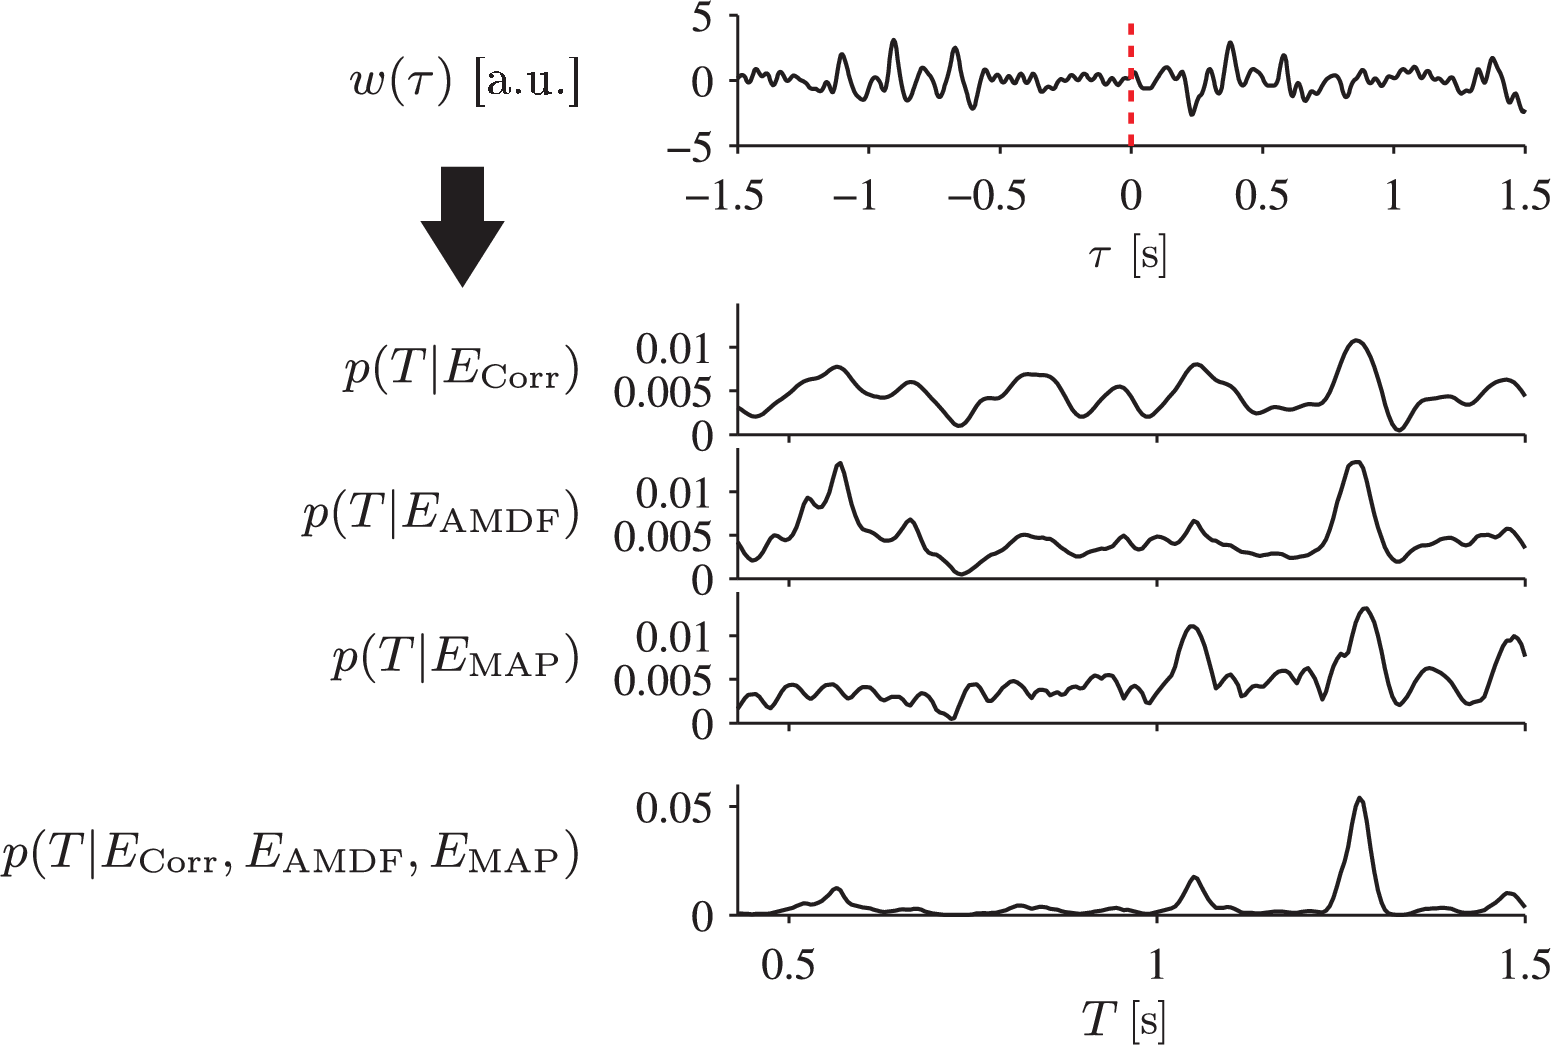
\includegraphics[width=0.7\textwidth]{pic/estimator-fusion.png}
		\caption[Intervallschätzer nach \citeauthor{Bruser2013}]{Die drei Intervallschätzer und ihre Fusionierung}
		\label{fig:estimator-fusion}
	\end{figure}
	
	\footcites[Vgl. zu diesem Absatz][]{Bruser2013}{Zink2017}

\section{Artefakterkennung}

	\subsection{Allgemein bei kardiorespiratorischen Signalen}

	\begin{itemize}
		\item Artefakte = irrelevante Signalteile mit variierender Amplitude, Frequenz und Dauer, die physiologiches Signal stören \footcite{Nizami2013}
		\item Ziel Beurteilung Signalqualität: nur die Teile des Signals, die Vitalparameter enthalten verarbeiten
		\item Bewegungsartefakte, Sensorstörungen etc nicht verarbeiten
		\item Quelle Störung irrelevant, aber medizinische Abnormalitäten dürfen nicht als gestörtes Signal klassifiziert werden
		\item Signalqualität oft mit so genannten Signal Quality Indices gemessen
		\item je nach SQI und Anwendungsfall verschiedene Aussagen
		\item \citeauthor{Sadek2016}: Unterscheidung in Bezug auf Signalqualität zwischen informativ und nicht informativ
		\item informativ: \textit{noise} und Signal von guter Qualität, Features können ohne weitere Verarbeitung extrahiert werden
		\item nicht informativ: Informationen mit Artefakten und noise vermischt, weitere Verarbeitung vor Extraktion Vitalparameter nötig oder Extraktion von physiologischen Eigenschaften unmöglich
		\item im klinischen Kontext genutzte Artefakterkennung oft durch relativ einfaches Preprocessing \footcite[Vgl.][]{Nizami2013}
		\item oft bestimmte Informationen direkt oder indirekt \textit{hard coded}, kann zum einen etwas wie Typ oder Frequenz der Daten sein, aber auch demographische Informationen über die Patient*innen wie Alter, Gewicht oder medizinischer Zustand\footcite[Vgl.][]{Nizami2013}
		\item Beispiel für Beurteilung der Signalqualität von anderen kardiorespiratorischen Signalen, in diesem Fall \ac{EKG} und \ac{PPG} in Abbildung, betrachtet werden 10-Sekunden-Fenster %TODO: einfügen
	\end{itemize}
	
	\begin{figure}[H]
		\centering
		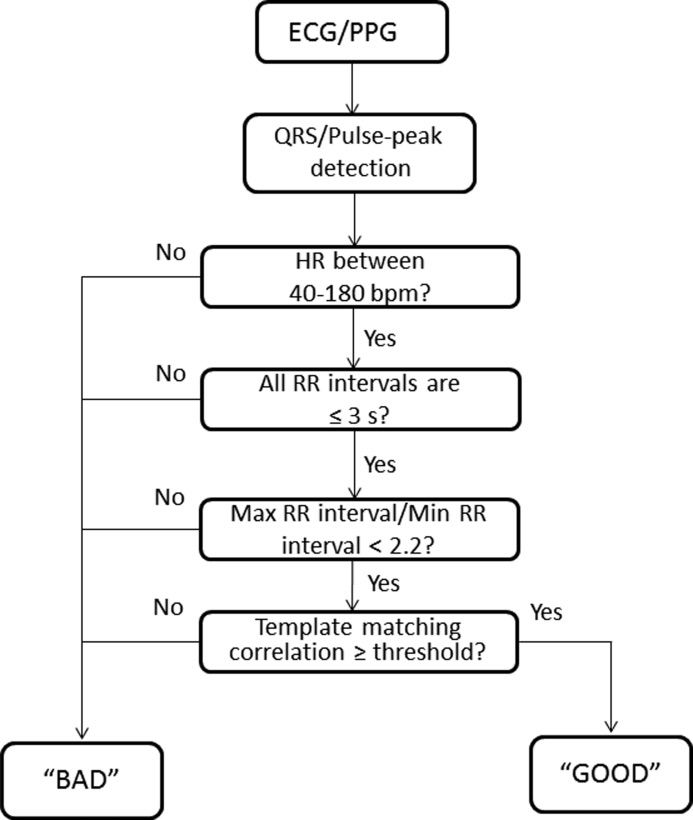
\includegraphics[width=0.7\textwidth]{pic/ad_flussdiagramm}
		\caption[Flussdiagramm eines Algorithmus zur Beurteilung der Signalqualität]{Flussdiagramm eines Algorithmus zur Beurteilung der Signalqualität\protect\footnotemark}
		\label{fig:ecg-ad}
		\footnotetext{Entnommen aus \cite{Orphanidou2015}.}
	\end{figure}
	
	
	\begin{itemize}
		\item erst Segmentierung der Herzschläge und dann 4 Kriterien überprüft -> reichen jeweils um Signal als schlecht zu klassifizieren
		\item Herzrate zwischen 40 und 180 Schlägen pro Minute? Abstand der Hochpunkte aufeinander folgender Herzschläge unter 3 Sekunden (kein Schlag fehlt?), Verhältnis maximales und minimales Schlag-zu-Schlag-Intervall kleiner als 2.2 (Begrenzung Veränderung Herzrate in untersuchtem 10-Sekunden-Fenster), Korrelation zu erstelltem Template höher als Schwellwert?
	\end{itemize}
	
	\subsection{Bei ballistokardiographischen Signalen}
	
	\begin{itemize}
		\item bei \ac{BKG} auch Artefakterkennung schwieriger als bei anderen kardiorespiratorischen Signalen: zusätzlich zur Variabilität bei Atmung Veränderungen bei Positionsänderungen -> vorher erstellte Templates werden obsolet
		\item Beispiele für Artefakte, einmal mit hoher, einmal mit niedriger Energie
		\item hohe Energie größere Bewegungen, leicht zu erkennen
	\end{itemize}
	
	\begin{figure}[H]
		\centering
		\begin{minipage}{0.45\linewidth}
      		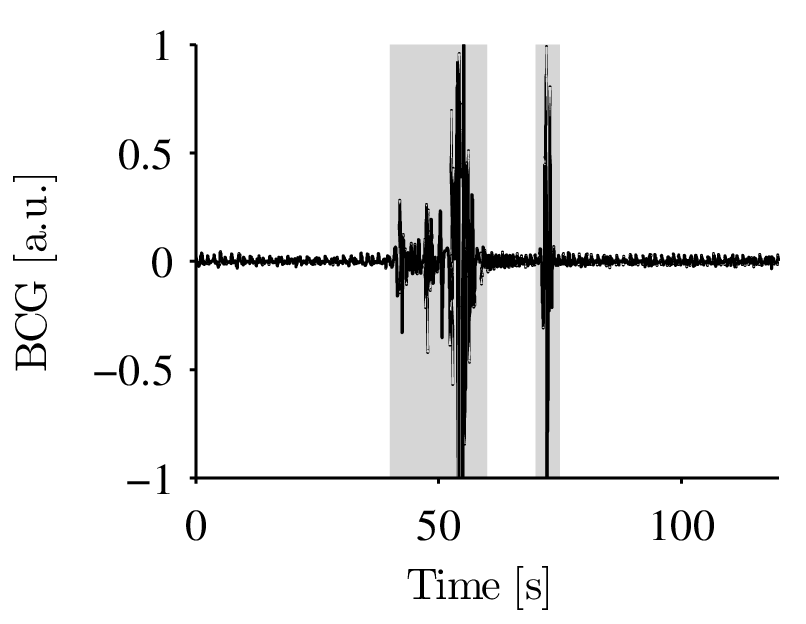
\includegraphics[width=\textwidth]{pic/high-energy-artifacts.png}
			\caption[Artefakte mit hoher Energie]{Artefakte mit hoher Energie}
			\label{fig:high-energy-artifact}
    	\end{minipage}
    	\hfill
    	\begin{minipage}{0.45\linewidth}
      		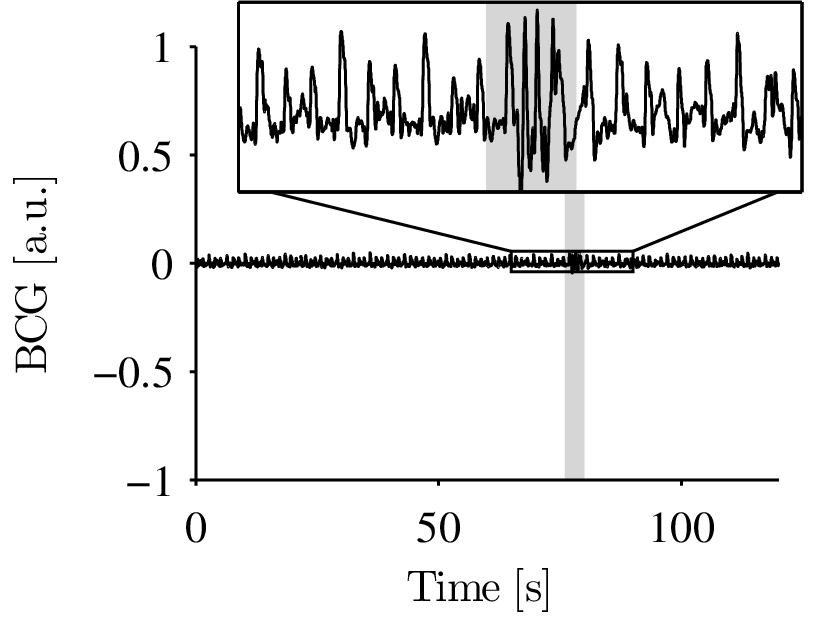
\includegraphics[width=\textwidth]{pic/low-energy-artifacts.png}
			\caption[Artefakte mit niedriger Energie]{Artefakte mit niedriger Energie}
			\label{fig:low-energy-artifact}
    \end{minipage}
		
	\end{figure}
	
	\begin{itemize}
		\item oft genutzt, dass Bewegungen stärkere Krafteinwirkungen verursachen, als Atmung und Herzschlag, das sind dann Artefakte mit hoher Energie
		\item bei Betrachtung verschiedener Ansätze zur Signalverarbeitung: Proband*innen oft angewiesen, sich möglichst wenig zu bewegen -> nicht realistisch für BKG-Aufnahmen in Betten
		\item \footcite{HoogAntink2020} festgestellt, dass bei Messsystemen in Betten besonders die Messung während des Tages große Signalteile von schlechter Qualität aufweisen, mehr als nachts, sichtbar ist z.B. auch Zeit des Mittagessens
		\item teils EKG-Referenz zur Artefakterkennung genutzt -> im \textit{unobtrusive} Kontext nicht zielführend
		\item im Folgenden ausgewählte Ansätze vorgestellt
	\end{itemize}

	\subsection{Schwellwertbasierte Artefakterkennung}
	
	In \citetitle{Pino2015} präsentieren \citeauthor{Pino2015} einen Ansatz für die Erkennung von Körperbewegungen für ein in einen Stuhl eingebettetes \ac{BKG}-Messsystem. Dafür werden über ein \textit{moving window} Maximum, Minimum, Standardabweichung und Mittelwert ermittelt und daraus 2 Schwellwerte berechnet:
	
	\begin{eqnarray*}
		&T_1 &= \frac{\text{max} + \text{min}}{2},\notag\\
		&T_2 &= \text{mean} + 1,1 * \text{std}.\notag
	\end{eqnarray*}
	
	Die Länge des \textit{moving window} ist mit 200 Samples bei einer Abtastrate von 200 Hz benannt. Untersucht wurden sowohl Freiwillige im Labor, als auch im Krankenhauswartezimmer für eine sehr kurze Messdauer von ein bis zwei Minuten. Mit diesem Ansatz wurde bei mehr als 50 \% der Laborgruppe eine \textit{Coverage} zwischen 87 \% und 95 \% erreicht. Die \textit{Coverage} der im Krankenhaus aufgenommenen Gruppe war bedeutend niedriger; hier lagen 50 \% der Messungen zwischen 48 \% und 95 \% \textit{Coverage} erreicht. Zu der Genauigkeit der Herzschlagdetektion auf den akzeptierten Signalteilen wird keine Aussage in Zahlen getroffen sondern nur der folgende Bland-Altman Graph gezeigt.
	
	\begin{figure}[H]
		\centering
		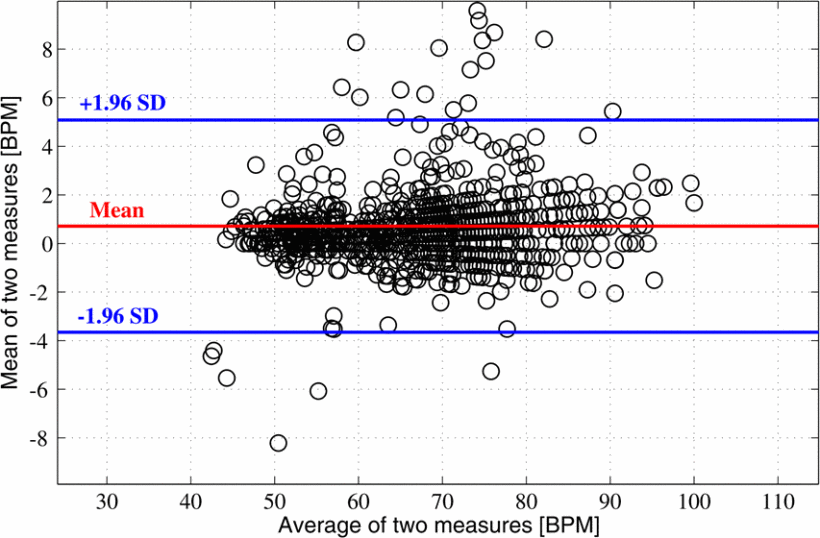
\includegraphics[width=0.7\textwidth]{pic/bland-altman-pino.png}
		\caption[Bland-Altman Graph zwischen von \ac{EKG} und \ac{BKG} berechneter \ac{HR}]{Bland-Altman Graph zwischen von \ac{EKG} und \ac{BKG} berechneter \ac{HR}}
		\label{fig:bland-altman-pino}
	\end{figure}
	
	Hier zeigt sich, dass beim Großteil des hier betrachteten Signals die \ac{HR} größtenteils mit einer Genauigkeit von $\pm$ Schläge pro Minute bestimmt werden konnte. Allerdings handelt es sich hier um im Sitzen aufgenommenes Signal, bei dem die Variabilität geringer ist als bei in Betten aufgenommenem \ac{BKG}.
	
	
	\subsection{Maschinelles Lernen mit statistischen Merkmalen}
	
	Ein Algorithmus zur Beurteilung der Signalqualität mittels maschinellen Lernens wird von \citeauthor{Sadek2016} im Paper \citetitle{Sadek2016} beschrieben. Betrachtet werden \ac{BKG}-Signale, die in einem Massagesessel aufgenommen werden, also ebenfalls im Sitzen aufgenommenes Signal, bei dem eine geringere Variabilität als in unserem Anwendungsfall erwartet wird.
	
	Die vorliegenden Daten wurden manuell von Expert*innen als informativ oder nicht informativ klassifiziert und in 10-Sekunden-Segmente, die sich nicht überlappen, aufgeteilt, die sich nicht überlappen. Insgesamt waren 58 \% der Daten als informativ und 42 \% als nicht-informativ gelabelt. Von diesen Segmenten wurden nach einer Bandpass-Filterung auf 1 bis 12 Hz 13 statistische Merkmale berechnet:
	\begin{itemize}
		\item Minimun
		\item Maximum
		\item Mittelwert
		\item Standardabweichung
		\item Schiefe
		\item Kurtosis
		\item Spannweite
		\item Interquartilspannweite
		\item mittlere absolute Abweichung
		\item Anzahl der Nulldurchgänge
		\item Varianz der lokalen Minima
		\item Varianz der lokalen Maxima
		\item Mittelwerte der Signalhüllkurve\footnote{Die Signalhüllkurve ist eine glatte Kurve, die die Extrema des Signals umreißt.}
	\end{itemize}
	
	Für fünf verschiedene Modelle des maschinellen Lernens wurden jeweils die besten Hyperparameter über Kreuzvalidierung auf den Trainingsdaten ermittelt und die Modelle anschließend mit diesen Hyperparametern trainiert. Anschließend wurden die Modelle auf unbekannten Daten getestet. Das Training und Testen wurde mit getauschten Gruppen wiederholt. Das beste Ergebnis wurde mit einem Random Forest erreicht: Die durchschnittliche Genauigkeit der Kreuzvalidierung betrug 98,13 \% bzw. 100 \% bei getauschten Gruppen. Auf dem Testset wurde eine Genauigkeit von 92,3 \% bzw. 97,99 \% erreicht. Weitere Evaluationsmetriken außer eine \textit{Confusion Matrix} für den besten Klassifkator sind nicht gegeben.
	
	Diese Ergebnisse sind sehr gut, allerdings muss bei der Einordnung beachtet werden, dass bei für die Kreuzvalidierung die Segmente zufällig verteilt wurden und nicht beachtet wurde, dass der Algorithmus für aussagekräftige Validierung einzelne Personen nicht darf. Dadurch ist die Performance auf gänzlich unbekannten Daten weiterhin nicht bekannt und vermutlich schlechter, als die Zahlen es hier vermuten lassen.
	
	\subsection{Ähnlichkeit der Intervallschätzer des CLIE-Algorithmus}
	
	Ein weiteres Maß für die Signalqualität basiert auf dem in \ref{CLIE} vorgestellten Algorithmus zur Intervallschätzung. Dieser \acl{SQI} misst, wie einig sich die drei Intervallschätzer sich. Wenn diese sich uneinig sind, ist der \ac{SQI} bei 0, je ähnlicher sich die Schätzungen sind, desto höher ist er. Für jedes Fenster $i$ wird er wie folgt berechnet: \[ q = \frac{E_f[n_{opt}, i]}{\sum E_f[n, i]} \]
	

\section{Messdaten}
	
	\subsection{Erfassung}
	
	\begin{itemize}
		\item aufgenommen in der Gefäßstation des Universitätskrankenhauses in Tampere in Finnland
		\item 14 Patient*innen wurden bis zu 24 h überwacht
		\item 2 weiblich, 12 männlich
		\item Durchschnittsalter: 69,57 Jahre
		\item nach verschiedenen gefäßchirurgischen Eingriffen
		\item durchschnittliche Messdauer: 17.7 h, range 4,46 bis 22,96 h
		\item EMFit QS Bettsensor, zwischen Matratze des Krankenhausbettes und Bettgestehl positioniert
		\item Samplingrate des EMFit QS Systems: 100 Hz, Bandpass-limitiert auf 1 bis 5 Hz
		\item Referenz EKG: Faros 360 5 lead Holter monitor, 1 kHz Abtastrate
		\item variabler Drift zwischen beiden Signalen % TODO: näher beschreiben
	\end{itemize}
	
	\subsection{Vorliegende Form}
	
	\begin{itemize}
		\item unbearbeitetes \ac{BKG}-Signal, abgesehen von der Bandpasslimitierung auf 1 bis 5 Hz
		\item unbearbeitetes 3-Kanal EKG Signal
		\item mit CLIE-Algorithmus detektierte Herzschläge, schon nach Qualität gefiltert mitsamt Brüser SQI, Länge und Länge des Herzschlages der EKG Referenz
		\item Vektoren, die den Drift der beiden Signale beschreiben, Form Sekunde \ac{BKG}-Signal und entsprechende Sekunde in \ac{EKG}-Referenz
	\end{itemize}
	
	\subsection{Verarbeitung und Datenstruktur}
	
	\begin{itemize}
		\item Datensatz von einem Patient besteht aus BKG Signal und EKG Referenz
		\item beides wird eingelesen, geprüft ob schon Detektion von Herzschlägen (Erkennen von R-Peaks bzw. CLIE Algorithmus schon durchgeführt wurde und als csv-Datei existiert
	\end{itemize}

	\subsection{Annotation der Daten}
	
	Die vorliegenden Daten sind nicht annotiert. Es ist im Rahmen dieser Arbeit nicht möglich, die Annotation durch Expert*innen durchführen zu lassen, weshalb auf das parallel aufgenommene \ac{EKG} zurückgegriffen wird.
	
	\begin{itemize}
		\item aufgrund des nicht-linearen Drifts der Daten herzschlaggenaue Synchronisierung schwierig
		\item Entscheidung Annotation von Bereichen von mehren Sekunden möglich zu machen
		\item Ablauf: existiert EKG Signal zu diesem Zeitpunkt, bei dem eine Herzfrequenz ermittelt werden konnte
		\item Berechnung dieser -> Anzahl der R-Peaks in diesem Bereich -1 geteilt durch den Abstand des letzten und des ersten Peaks
		\item Berechnung \ac{BKG}-Herzfrequenz: Durchschnitt der geschätzten Längen der erkannten Peaks im Bereich
		\item Annotation anhand von relativer oder absoluter Abweichung der beiden
	\end{itemize}
	

